%%%%%%%%%%%%%%%%%%%%%%%%%%%%%%%%%%%%%%%%
%% Slides : Bayes basics ("bayesics") %%
%%%%%%%%%%%%%%%%%%%%%%%%%%%%%%%%%%%%%%%%

%% PREAMBLE
%% Define document class and basic options
\documentclass{beamer}
%\setlength{\parindent}{0pt}

%% Load packages
\usepackage{palatino}
\usepackage{amsfonts}
\usepackage{amsmath}
%\usepackage{url}
\usepackage{hyperref}
%\usepackage{listings}
\usepackage{verbatim}
\usepackage[utf8]{inputenc} %% For french
\usepackage{tikz} %% For drawing (eg, Venn diagrams)
\usefonttheme{serif}

\hypersetup{
	colorlinks=true,
	linkcolor=blue,
	citecolor=red,
	filecolor=blue,
	urlcolor=blue
}

\usetheme{Madrid}

%% Basic info
\title{Introduction à la pensée et aux méthodes bayésiennes}
%\subtitle{}
\author{Roy Nitulescu\inst{1}}

\institute
{
    \inst{1}%
    CITADEL\\
    CR-CHUM
}

\date[UdeM, Sept. 28, 2022]{Université de Montréal, Sept. 28, 2022}

\AtBeginSection[]
{
    \begin{frame}
        \frametitle{Table des matières}
        \tableofcontents[currentsection]
    \end{frame}
}

\AtBeginSubsection[]
{
    \begin{frame}
        \frametitle{Table des matières}
        \tableofcontents[currentsubsection]
    \end{frame}
}


%% BEGIN DOCUMENT
\begin{document}

%%%%
%% Slides
%%%%

\frame{\titlepage}

\begin{frame}
    \frametitle{Épigraphe}
    ``La probabilité est le concept le plus important de la science moderne,
    d'autant plus que personne n'a la moindre idée de ce qu'elle signifie.'' -- Bertrand Russell, 1929
\end{frame}


\begin{frame}
    \frametitle{Préambule}
    
    Le code source pour cette présentation ce trouve ici:

    \vfill

    \url{https://github.com/rnitulescu/bayesics}
\end{frame}


\begin{frame}
    \frametitle{Table des matières}
    \tableofcontents
\end{frame}


%%%%
%% Motivation
%%%%

\section{Motivation}

\begin{frame}
    \frametitle{La dualité du concept de probabilité}

    De par son origine, le concept a une \textbf{dualité}\footnote{
    Hacking, Ian (1975). \emph{The emergence of probability:
    A philosophical study of early ideas about probability,
    induction and statistical inference}. Cambridge University Press.
    }

    \pause

    \vfill

    \begin{enumerate}
      \item \textbf{Aléatoire}
        \begin{itemize}
          \item Fréquence (la limite d'une fréquence relative dans une séquence infinie)
          \item Propension (une propriété intrinsèque d'objets ou de situations)
        \end{itemize}

      \pause

      \item \textbf{Épistémique}
        \begin{itemize}
          \item Logique (le degré de soutien ou de confirmation qu'un élément d'évidence confère à une hypothèse donnée)
          \item Subjectif (crédibilité ou degré de croyance subjectif)
        \end{itemize}
    \end{enumerate}    
\end{frame}


\begin{frame}
    \frametitle{Allocation de crédibilité}
    \textbf{L'inférence bayésienne} peut être résumée ainsi: \pause
    \begin{itemize}
      \item C'est la \textbf{réallocation de crédibilité} parmi toutes les possibilités hypothétiques
            (mutuellement exclusives et exhaustives)
      \pause
      \item Les possibilités sont les valeurs potentielles de \textbf{paramètres} dans un modèle mathématique
    \end{itemize}
\end{frame}


\begin{frame}
    \frametitle{Allocation de crédibilité}
    \textbf{Exemple abstrait:}
    
    \begin{figure}
      \centering
      \includegraphics[scale=0.5]{images/credibility.eps}
      \caption{Allocation et réallocation de crédibilité}
    \end{figure}
\end{frame}


\begin{frame}
    \frametitle{Allocation de crédibilité}
    \textbf{Exemple concret:\footnote{
      Exemple pris de Kruschke, J. K.(2015). \emph{Doing Bayesian data analysis: A tutorial with R, JAGS, and Stan}.
            Academic Press, pp 20-21.
    }}
    Une usine produit des ballons ronds de différentes tailles (diamètre = 1 dm, 2 dm, 3 dm, ou 4 dm) \pause
    \begin{itemize}
      \item Mais il y a de la variation dans les tailles exactes, en pratique
      \pause
      \item Par exemple, la taille de chaque ballon suit approximativement une loi normale avec
            taille \textbf{moyenne} de 1, 2, 3, ou 4 dm et \textbf{écart type} de 1.16 dm
      \pause
      \item Supposons que nous avons commandé trois ballons d'une même taille (diamètre = 2 dm),
            mais que nous avons reçu trois ballons avec les tailles suivantes: 1.77, 2.23, et 2.70 dm.
      \pause
      \item Quelle est la probabilité que les trois ballons soient du type avec diamètre = 2 dm?
            Même question pour les autres tailles (1, 3, 4 dm). Finalement, quelle est la
            taille la plus crédible?
    \end{itemize}
\end{frame}


\begin{frame}
    \frametitle{Allocation de crédibilité}
    On reviendra à cet exemple plus tard (vous devrez le résoudre comme exercice).

    \pause

    \vfill

    Pour répondre à cette question, nous avons besoin d'un peu de théorie.

    \pause

    \vfill

    Mais avant: une peu d'intuition.
\end{frame}


%%%%
%% Intuition
%%%%

\section{Intuition}

\begin{frame}
    \frametitle{Exemple: diagnostic de maladie\footnote{
        Emprunté et modifié d'un exemple pris dans: Devlin, Keith (2010).
        \emph{The unfinished game: Pascal, Fermat, and the seventeenth-century letter that made the world modern.}
        Basic Books, pp 139-142.
    }}
    Supposons que vous avez reçu un résultat positif pour un test diagnostic d'une maladie rare.
    Quelle est la probabilité que vous ayiez cette maladie ($\boldsymbol{H}$),
    sachant que le résultat du test est positif ($\boldsymbol{E}$)?

    \pause

    \vfill

    Voici les faits:
    \begin{itemize}
      \item Prévalence: Parmi \textbf{10,000} individus, \textbf{100} ont la maladie (donc, \textbf{9,900} ne l'ont pas)
      \pause
      \item Sensibilité du test: Parmi les \textbf{100} malades,
            \textbf{95} reçoivent un diagnostic positif (donc, \textbf{5} faux négatifs)
      \pause
      \item Spécificité du test: Parmi les \textbf{9,900} en santé,
            \textbf{7,821} reçoivent un diagnostic négatif (donc, \textbf{2,079} faux positifs)
    \end{itemize}
\end{frame}


\begin{frame}
    \frametitle{Exemple: diagnostic de maladie}
    \begin{figure}
      \centering
      \scalebox{0.75}{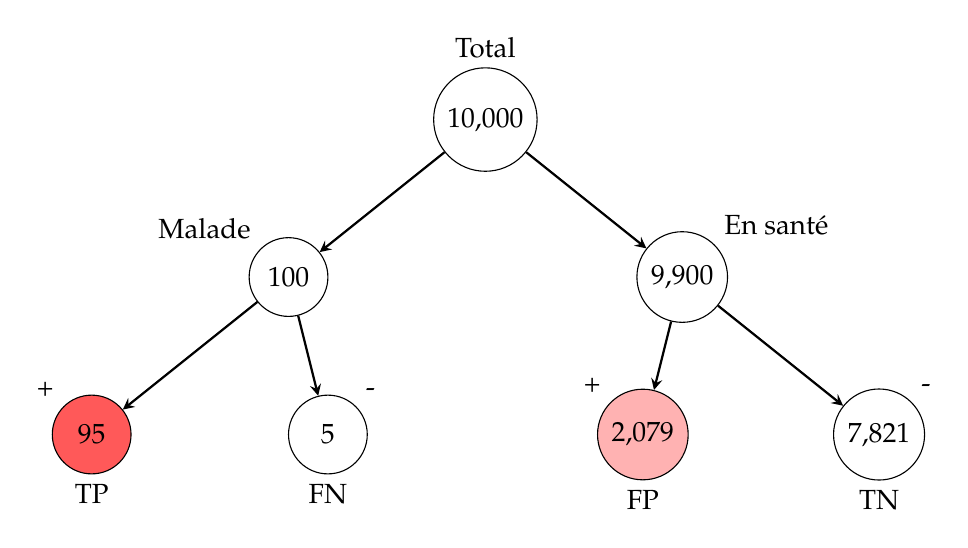
\begin{tikzpicture}
    \tikzstyle{arrow} = [thick,->,>=stealth]
    % Top bubble
    \node [draw, circle, minimum size=1cm, text centered, label={90:Total}] (Top) at (0,5) {10,000};

    % Lower left bubble
    \node [draw, circle, minimum size=1cm, text centered, label={135:Malade}] (Diseased) at (-2.5,3) {100};
    \draw [arrow] (Top) -- (Diseased);

    % Lower right bubble
    \node [draw, circle, minimum size=1cm, text centered, label={45:En santé}] (NonDiseased) at (2.5,3) {9,900};
    \draw [arrow] (Top) -- (NonDiseased);

    % Bottom extreme left
    \node [draw, circle, minimum size=1cm, text centered, label={135:+}, label={-90:TP}, fill=red!65] (TP) at (-5,1) {95};
    \draw [arrow] (Diseased) -- (TP);

    % Bottom mid left
    \node [draw, circle, minimum size=1cm, text centered, label={45:-}, label={-90:FN}] (FN) at (-2,1) {5};
    \draw [arrow] (Diseased) -- (FN);

    % Bottom mid right
    \node [draw, circle, minimum size=1cm, text centered, label={135:+}, label={-90:FP}, fill=red!30] (FP) at (2,1) {2,079};
    \draw [arrow] (NonDiseased) -- (FP);

    % Bottom extreme right
    \node [draw, circle, minimum size=1cm, text centered, label={45:-}, label={-90:TN}] (TN) at (5,1) {7,821};
    \draw [arrow] (NonDiseased) -- (TN);
\end{tikzpicture}

}
    \end{figure}

    \pause

    La proportion des patients avec un test positif qui sont véritablement malades est de
    \[\frac{95}{95 + 2079} = 0.044 .\]
\end{frame}


\begin{frame}
    \frametitle{Exemple: diagnostic de maladie (en probabilités)}
    \begin{figure}
      \centering
      \scalebox{0.65}{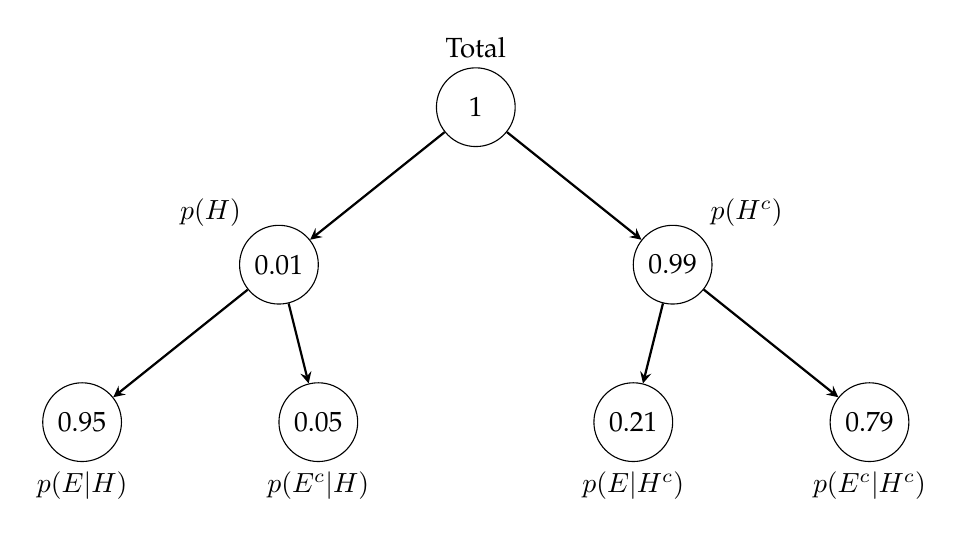
\begin{tikzpicture}
    \tikzstyle{arrow} = [thick,->,>=stealth]
    % Top bubble
    \node [draw, circle, minimum size=1cm, text centered, label={90:Total}] (Top) at (0,5) {1};

    % Lower left bubble
    \node [draw, circle, minimum size=1cm, text centered, label={135:$p(H)$}] (Diseased) at (-2.5,3) {0.01};
    \draw [arrow] (Top) -- (Diseased);

    % Lower right bubble
    \node [draw, circle, minimum size=1cm, text centered, label={45:$p(H^c)$}] (NonDiseased) at (2.5,3) {0.99};
    \draw [arrow] (Top) -- (NonDiseased);

    % Bottom extreme left
    \node [draw, circle, minimum size=1cm, text centered, label={-90:$p(E | H)$}] (TP) at (-5,1) {0.95};
    \draw [arrow] (Diseased) -- (TP);

    % Bottom mid left
    \node [draw, circle, minimum size=1cm, text centered, label={-90:$p(E^c | H)$}] (FN) at (-2,1) {0.05};
    \draw [arrow] (Diseased) -- (FN);

    % Bottom mid right
    \node [draw, circle, minimum size=1cm, text centered, label={-90:$p(E | H^c)$}] (FP) at (2,1) {0.21};
    \draw [arrow] (NonDiseased) -- (FP);

    % Bottom extreme right
    \node [draw, circle, minimum size=1cm, text centered, label={-90:$p(E^c | H^c)$}] (TN) at (5,1) {0.79};
    \draw [arrow] (NonDiseased) -- (TN);
\end{tikzpicture}

}
    \end{figure}

    \pause

    Si on suit l'arbre de façon analogique:
    \[p(H | E) = \frac{(0.95)(0.01)}{(0.95)(0.01) + (0.21)(0.99)}\]
    \pause
    \[ = \frac{p(E | H) \, p(H)}{p(E | H) \, p(H) + p(E | H^c) \, p(H^c)} = \frac{p(E | H) \, p(H)}{p(E)}\]
\end{frame}


%%%%
%% Théorie
%%%%

\section{Théorie}

%% Théorie des ensembles (révision)

\subsection{Théorie des ensembles (révision)}

\begin{frame}
  \frametitle{Théorie des ensembles (version naïf)}
  \begin{itemize}
    \item Un ensemble est une collection d'éléments (ex: $X = \{1,2,3,4,5,6\}$)
    \pause
    \item Un sous-ensemble, $A \subset X$, est aussi un ensemble (ex: $A = \{1,3,5\}$)
    \pause
    \item Opérations de base:
    \begin{itemize}
      \item Union: $A \cup B$ contient chaque élément ce trouvant dans $A$ \emph{ou} $B$
      \pause
      \item Intersection: $A \cap B$ contient chaque élément ce trouvant dans $A$ \emph{et} $B$
      \pause
      \item Complément: $A^c$ contient chaque élément qui ne se trouve \emph{pas} dans $A$ (sous l'hypothèse d'un ensemble universel)
    \end{itemize}
  \end{itemize}
\end{frame}


%% Théorie de la probabilité discrète (révision)

\subsection{Probabilités discrètes (révision)}

\begin{frame}
    \frametitle{Espace d'échantillonnage, $S$}
    \begin{itemize}
      \item L'espace, $S$, qui contient toutes les issues possible d'une expérience
      \pause
      \item Toutes ces possibilités sont mutuellement exclusives et exhaustives
      \pause
      \item Chaque \textbf{issue} a une \textbf{masse} de probabilité
      \pause
      \item On définit un \textbf{événement}, $A$, comme étant un sous-ensemble de $S$ (ex: ``rouler un nombre impair'' = $\{1,3,5\}$)
      \pause
      \item On calcule la probabilité d'un événement en comptant le nombre d'éléments dans $A$ et en divisant par le nombre d'éléments dans $S$
    \end{itemize}
\end{frame}


\begin{frame}
    \frametitle{Les axiomes de Kolmogorov}
    \begin{itemize}
      \item $\textrm{(K1)} \, \, p(A) \geq 0, \textrm{où} \, \, A \subset S$
      \pause
      \item $\textrm{(K2)} \, \, p(S) = 1$
      \pause
      \item $\textrm{(K3)} \, \, p(\bigcup_{i=1}^{\infty} A_i) = \sum_{i=1}^{\infty} p(A_i)$, où les ensembles $A_i$ sont mutuellement exclusifs
    \end{itemize}
\end{frame}


\begin{frame}
    \frametitle{Propriétés de la probabilité (négation)}
    A partir des axiomes, on peut dériver maintes propriétés et relations. Voici un exemple.\\
    \pause
    \[p(S) = p(A \cup A^c) = p(A) + p(A^c) = 1\]
    \pause
    Donc,
    \[p(A^c) = 1 - p(A)\]
    \pause
    \begin{figure}
      \centering
      \scalebox{1}{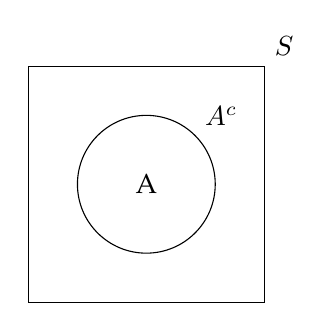
\begin{tikzpicture}
    % Sample space
    \node [draw,
    rectangle,
    minimum size =3cm,
    label={45:$S$}] (S) at (0,0){};

    % Set A
    \node [draw,
    circle,
    minimum size =1.75cm, text centered,
    label={45:$A^c$}] (A) at (0,0){A};
\end{tikzpicture}

}
      \caption{Diagramme de Venn représentant la négation (complément)}
    \end{figure}    
\end{frame}


\begin{frame}
    \frametitle{Propriétés de la probabilité (additivité)}
    On peut généraliser:

    \pause

    \vfill

    Si 
    \[A_1 \cup A_2 \cup \ldots \cup A_n = S,\]
    où les ensembles $A_i$ sont mutuellement exclusifs,
    \[\sum_{i=1}^{n} p(A_i) = 1.\]
\end{frame}


%% Skipping, since not needed for this lecture (though a standard basic result)
%\begin{frame}
%    \frametitle{Propriétés de la probabilité (Union)\footnote{
%        Si $A$ et $B$ sont mutuellement exclusifs, $p(A \cap B) = 0$
%    }}
%    \[p(A \cup B) = p(A) + p(B) - p(A \cap B)\]
%    \pause
%    \begin{figure}
%      \centering
%      \scalebox{1}{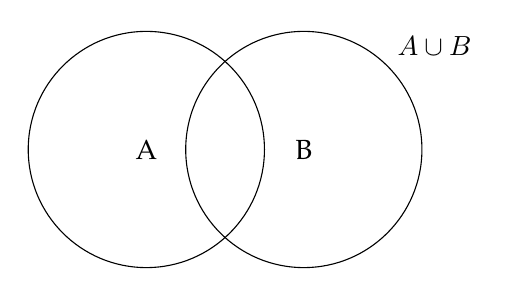
\begin{tikzpicture}
    % Set A
    \node [draw,
    circle,
    minimum size =3cm, text centered] (A) at (0,0){A};

    % Set B
    \node [draw,
    circle,
    minimum size =3cm, text centered,
    label={45:$A \cup B$}] (B) at (2,0){B};
\end{tikzpicture}

}
%      \caption{Diagramme de Venn représentant $p(A \cup B)$}
%    \end{figure}    
%\end{frame}


\begin{frame}
    \frametitle{Probabilité d'intersection}
    $A = \{2,4,6\}$ et $B = \{3,6\}$, donc $A \cap B = \{6\}$ et $p(A \cap B) = 1/6$.\\
    \vfill
    \pause
    Si $A$ et $B$ sont mutuellement exclusifs, $p(A \cap B) = 0$    
    \begin{figure}
      \centering
      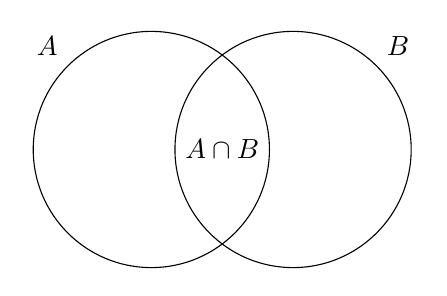
\begin{tikzpicture}
    % Set A
    \node [draw,
    circle,
    minimum size =3cm,
    label={135:$A$}] (A) at (0,0){};

    % Set B
    \node [draw,
    circle,
    minimum size =3cm,
    label={45:$B$}] (B) at (1.8,0){};

    % Set intersection label
    \node at (0.9,0) {$A\cap B$};
\end{tikzpicture}


      \caption{Diagramme de Venn représentant $p(A \cap B)$}
    \end{figure}
\end{frame}


\begin{frame}
    \frametitle{Probabilité jointe}
    Pour l'instant on n'a regardé que des probabilités univariés. Mais on peut avoir des probabilités multivariés également.
    Exemple: un tableau croisé.
    \pause
    \begin{table}[h!]
      \centering
      \begin{tabular}{|l|c|c|c|c|}
        \hline
        Cheveux & Noirs & Bruns & Roux & Blonds \\
        \hline\hline
        Yeux bruns & 11 & 20 & 4 & 1 \\
        Yeux bleus & 3 & 14 & 3 & 16 \\
        Yeux verts & 1 & 5 & 2 & 3 \\
        \hline
      \end{tabular}
      \caption{Tableau croisé (distribution bivarié)}
    \end{table}
    \pause
    A partir de cette table, on peut calculer des probabilités de la forme $\textbf{p(x, y)}$ (dites \emph{jointes}),
    où $x$ représente la couleur des yeux et $y$ représente la couleur des cheveux.
\end{frame}


\begin{frame}
    \frametitle{Probabilité marginale}
    A partir du même tableau croisé, on peut également calculer les probabilités \emph{marginaux} en prenants des sommes comme suit:
    \pause
    \[p(x) = \sum_y p(x,y)\]
    \pause
    et
    \[p(y) = \sum_x p(x,y).\]
\end{frame}


\begin{frame}
    \frametitle{Probabilité conditionnelle I}
    Dans le contexte des axiomes de Kolmogorov, on définit la probabilité conditionnelle ainsi:
    \[p(A | B) = \frac{p(A \cap B)}{p(B)}.\]
    \pause
    \[\textrm{Donc,} \, \, p(A \cap B) = p(A | B) \, p(B).\]
    %% Below is WRONG. Careful to move it where it applies correctly to bivariate case...
    %\pause
    %\[\textrm{Si A et B sont indépendents,} \, \, p(A | B) = p(A).\]
    %\pause
    %\[\textrm{Donc,} \, \, p(A \cap B) = p(A) \, p(B).\]
    \pause
    \vfill
    Notez: dans d'autres systèmes axiomatiques de probabilité, par exemple dans le système à De Finetti,
    la probabilité conditionnelle est un concept de base, et donc, la deuxième équation serait un axiome dans
    ce système-là.
\end{frame}


\begin{frame}
    \frametitle{Probabilité conditionnelle II}
    On peut également exprimer les probabilités conditionnelles pour le cas bivarié.

    \vfill

    \pause

    Par exemple, si nous prenons notre exemple de tout-à-l'heure, la probabilité d'avoir
    les yeux bleus \emph{et} les cheveux bruns ($p(\textrm{`yeux bleus'} \cap \textrm{`cheveux bruns'})$) peut
    être exprimée comme une probabilité jointe:
    
    \pause

    \[p(x=\textrm{`yeux bleus'}, y=\textrm{`cheveux bruns'}).\]

    \pause

    \vfill

    Donc, on peut définir la probabilité conditionnelle ainsi:
    \[p(x | y) = \frac{p(x,y)}{p(y)}.\]
\end{frame}


\begin{frame}
    \frametitle{Indépendance de variables aléatoires}
    On définit la propriété d'indépendance de deux variables aléatoires ainsi.
    Deux variables aléatoires, $x$ et $y$, sont dites indépendantes si:
    \[p(x,y) = p(x) \, p(y).\]
    \pause
    \vfill
    Dans une perspective plus épistémique de la probabilité, on peut aussi définir cette propriété ainsi.
    Deux variables aléatoires, $x$ et $y$, sont dites indépendantes si:
    \[p(x|y) = p(x).\]
    \pause
    \vfill
    Alors, cela impliquerait que $p(x,y) = p(x) \, p(y)$ puisque $p(x|y) = p(x,y) / p(y)$.
\end{frame}


\begin{frame}
    \frametitle{Loi de probabilité totale I}
    \begin{figure}
      \centering
      \begin{tikzpicture}
    % Hypothesis is true
    \node [draw,
    rectangle,
    minimum size =3cm,
    label={135:$H$}] (H) at (-1.5,0){};

    % Hypothesis is false
    \node [draw,
    rectangle,
    minimum size =3cm,
    label={45:$H^c$}] (Hc) at (1.5,0){};

    % Set E for evidence is true
    \node [draw,
    circle,
    minimum size =2.5cm,
    label={145:$E$}] (E) at (0,0){};
\end{tikzpicture}


      \caption{Diagramme de Venn représentant loi de probabilité totale}
    \end{figure}
    \pause
    \[p(E) = p(E \cap H) + p(E \cap H^c)\]
    \[ = p(E | H) \, p(H) + p(E | H^c) \, p(H^c)\]
\end{frame}


\begin{frame}
    \frametitle{Loi de probabilité totale II}
    On peut généraliser:

    \pause

    \vfill

    Si 
    \[p(H_1) + p(H_2) + \ldots + p(H_n) = 1,\]
    où les ensembles $H_i$ sont mutuellement exclusifs,
    \pause
    \[p(E) = \sum_{i=1}^{n} p(E \cap H_i)\]
    \pause
    \[= \sum_{i=1}^{n} p(E | H_i) \, p(H_i).\]
\end{frame}


%% Théorie de la probabilité continue (révision)

\subsection{Probabilités continues (révision)}

\begin{frame}
    \frametitle{Masse et densité de probabilité}
    \begin{figure}
      \centering
      \includegraphics[scale=0.60]{images/mass_v_density.eps}
    \end{figure}
\end{frame}


\begin{frame}
    \frametitle{Espace d'échantillonnage}
    \begin{itemize}
      \item Pour une variable continue, l'espace d'échantillonnage peut être l'ensemble des nombres réels
      \pause
      \item Pour chaque issue dans cet espace, on ne peut que mesurer sa \textbf{densité} de probabilité
      \pause
      \item Pour mesurer une masse, il faut prendre l'intégrale de la fonction
            de densité sur une intervalle de son espace d'échantillonnage
    \end{itemize}
\end{frame}


\begin{frame}
    \frametitle{Propriétés de la probabilité (additivité)}
    Si $p_X(x)$ est la fonction de densité de probabilité de $x$,
    \[\int_X p_X(x) \, dx = 1.\]
    \vfill
    \pause
    Ceci suit directement des axiomes (K2) et (K3), si on partitionne l'espace d'échantillonnage
    en petits intervalles et prenons la somme Riemann. Dans la limite que les intervalles sont infiniment
    petits, la somme converge à l'intégrale de Riemann, ce qui donne l'identité en haut.
\end{frame}


\begin{frame}
    \frametitle{Probabilité jointe}
    Si $x$ et $y$ sont indépendants,
    \[p_{X,Y}(x,y) = p_X(x) \, p_Y(y).\]
    \pause
    De façon similaire, si $x$ et $y$ sont indépendants
    conditionnellement sur une autre variable, $z$,
    \[p_{X,Y|Z}(x,y|z) = p_{X|Z}(x|z) \, p_{Y|Z}(y|z).\]
\end{frame}


\begin{frame}
    \frametitle{Exemples de distributions jointes continues}
    \begin{figure}
      \centering
      \includegraphics[scale=0.60]{images/joint_densities.eps}
    \end{figure}
\end{frame}


\begin{frame}
    \frametitle{Relations entre probabilité jointe, marginale, et conditionnelle}
    \[\textrm{Marginale:} \, \, \, p_X(x) = \int_Y p_{X,Y}(x,y) \, dy\]
    \pause
    \[\textrm{Conditionnelle:} \, \, \, p_{X|Y}(x|y) = \frac{p_{X,Y}(x,y)}{p_Y(y)}\]
    \pause
    \[\textrm{Jointe:} \, \, \, p_{X,Y}(x,y) = p_{X|Y}(x|y) \, p_Y(y)\]
\end{frame}


\begin{frame}
    \frametitle{Loi de probabilité totale (version continue)}
    Si
    \[\int_Y p_Y(y) \, dy = 1,\]
    \pause
    \[p_X(x) = \int_{Y} p_{X,Y}(x, y) \, dy\]
    \pause
    \[= \int_{Y} p_{X|Y}(x | y) \, p_Y(y) \, dy.\]
\end{frame}


%% Théorie bayésienne

\subsection{Théorie bayésienne}

\begin{frame}
    \frametitle{Le théorème de Bayes (probabilités discrètes)}
    Le théorème suit directement de la définition de probabilité conditionnelle:

    \pause

    \[p(A \cap B) =  p(A | B) \, p(B) \,\,\, \pause \textrm{ et } \,\,\, p(B \cap A) =  p(B | A) \, p(A)\]
    \pause
    \[\textrm{Et puisque } \,\,\, p(A \cap B) = p(B \cap A)\]
    \pause
    \[\textrm{Il suit que } \,\,\, p(A | B) \, p(B) = p(B | A) \, p(A)\]
    \pause
    \[\textrm{Donc } \,\,\, p(A | B) = \frac{p(B | A) \, p(A)}{p(B)}\]
    
    Voilà!
\end{frame}


\begin{frame}
    \frametitle{Le théorème de Bayes (probabilités continues)}
    Le théorème suit directement de la définition de la densité conditionnelle:

    \pause

    \[p_{X|Y}(x|y) = \frac{p_{X,Y}(x,y)}{p_Y(y)} \,\,\, \pause \textrm{ et }\]
    \[p_{Y|X}(y|x) = \frac{p_{X,Y}(x,y)}{p_X(x)}\]
    \pause
    \[\textrm{Donc, il suit que } \,\,\, p_{X|Y}(x|y) \, p_Y(y) = p_{Y|X}(y|x) \, p_X(x)\]
    \pause
    \[\textrm{Ce qui implique que } \,\,\, p_{X|Y}(x|y) = \frac{p_{Y|X}(y|x) \, p_X(x)}{p_Y(y)}\]

    Voilà!
\end{frame}


%%%%
%% Applications
%%%%

\section{Applications}

\begin{frame}
    \frametitle{Exemple: mesurer son poids}
    Supposons que vous voulez mesurer votre poids, mais votre balance
    est très imprécise (mais non-biaisé). Comment inférer son poids à partir de plusieurs mesures?

    \pause

    \vfill

    \textbf{Le modèle}

    \[y_i \sim \textrm{N}(\mu, \sigma), \, \, \, i = 1, \ldots, n.\]

    \pause

    \begin{itemize}
      \item On prends $\boldsymbol{n}$ mesures de notre poids, $\boldsymbol{y_i}$
      \pause
      \item Les mesures suivent une loi normale avec moyenne, $\boldsymbol{\mu}$,
            inconnue et écart-type, $\boldsymbol{\sigma}$, connue
      \pause
      \item Disons que $\boldsymbol{n} = 5$, $\boldsymbol{\vec{y}} = (149, 127, 141, 130, 160)$, en livres,
            que $\boldsymbol{\sigma} = 10$, et que notre \emph{a priori} pour $\boldsymbol{\mu}$
            est $\boldsymbol{\mu} \sim \textrm{N}(136, 12)$
      \pause
      \item Finalement, on émet aussi l'hypothèse que les mesures de poids sont indépendantes
            conditionnellement sur le paramètre, $\boldsymbol{\mu}$
    \end{itemize}
\end{frame}


\begin{frame}
    \frametitle{Exemple: mesurer son poids}
    \textbf{Solution}

    \vfill

    Nous voulons estimer $p(\mu | \vec{y})$

    \pause

    \vfill

    D'après le théorème de Bayes

    \[p(\mu | \vec{y}) = \frac{p(\vec{y} | \mu) \, p(\mu)}{p(\vec{y})} 
      = \frac{p(\vec{y} | \mu) \, p(\mu)}{\int_{-\infty}^{+\infty} p(\vec{y} | \mu) \, p(\mu) \, d\mu} \, ,\]

    \pause

    et puisque les mesures de poids sont indépendants conditionnellement sur $\boldsymbol{\mu}$,

    \[p(\vec{y} | \mu) = \prod_{i=1}^{n} p(y_i | \mu) \, .\]
\end{frame}


\begin{frame}
    \frametitle{Exemple: mesurer son poids}
    Donc, les composantes du modèle sont:

    \pause

    \vfill

    \textbf{La vraisemblance (``likelihood'')}

    \[\prod_{i=1}^{n} \textrm{N}(y_i | \mu, 10)\]

    \pause

    \vfill

    \textbf{Le \emph{a priori} (``prior'')}

    \[\textrm{N}(\mu | 136, 12)\]

    \pause

    \vfill

    \textbf{La vraisemblance marginale (``marginal likelihood'')}

    \[\int_{-\infty}^{+\infty} \prod_{i=1}^{n} \textrm{N}(y_i | \mu, 10) \, \textrm{N}(\mu | 136, 12) \, d\mu\]
\end{frame}


\begin{frame}[fragile]
    \frametitle{Exemple: mesurer son poids}
    \textbf{Code R}
    \fontsize{9}{11}\selectfont
    \verbatiminput{../R/examples/weight_pt1.R}
\end{frame}


\begin{frame}[fragile]
    \frametitle{Exemple: mesurer son poids}
    \textbf{Code R}
    \fontsize{9}{11}\selectfont
    \verbatiminput{../R/examples/weight_pt2.R}
\end{frame}


\begin{frame}[fragile]
    \frametitle{Exemple: mesurer son poids}
    \textbf{Code R}
    \fontsize{9}{11}\selectfont
    \verbatiminput{../R/examples/weight_pt3.R}
\end{frame}


\begin{frame}
    \frametitle{Exemple: mesurer son poids}
    \textbf{Résultats:}
    \begin{figure}
      \centering
      \includegraphics[scale=0.60]{images/weight.eps}
    \end{figure}
\end{frame}


\begin{frame}
    \frametitle{Exemple: mesurer son poids}
    Et si on utilisait une méthode fréquentiste?

    \pause

    \vfill

    \[\mu = \bar{y} = \frac{\sum_{i=1}^{n} y_i}{n} = 141\]

    \pause

    \vfill

    \[\sigma_{\bar{y}} = \sqrt{\frac{\left(\frac{\sum_{i=1}^{n} (y_i - \bar{y})^2}{n-1}\right)}{n}} = 6.1\]

    \pause

    \vfill

    Donc, notre \emph{a priori} nous a aidé à diminuer l'écart type de notre estimé de $\boldsymbol{\mu}$
    de 6.1 à 4.25.
\end{frame}


\begin{frame}
    \frametitle{Exemple: retour aux ballons}
    Et maintenant c'est à votre tour de résoudre un problème plus simple que ce dernier exemple.

    \pause

    \vfill

    Une usine produit des ballons ronds de différentes tailles (diamètre = 1 dm, 2 dm, 3 dm, ou 4 dm) \pause
    \begin{itemize}
      \item Mais il y a de la variation dans les tailles exactes, en pratique
      \pause
      \item Par exemple, la taille de chaque ballon suit approximativement une loi normale avec
            taille \textbf{moyenne}, $\boldsymbol{\mu}$, de 1, 2, 3, ou 4 dm et \textbf{écart type} de 1.16 dm
      \pause
      \item Supposons que nous avons commandé trois ballons d'une même taille (diamètre = 2 dm),
            mais que nous avons reçu trois ballons avec les tailles suivantes: 1.77, 2.23, et 2.70 dm.
      \pause
      \item Quelle est la probabilité que les trois ballons soient du type avec diamètre = 2 dm?
            Même question pour les autres tailles (1, 3, 4 dm). Finalement, quelle est la
            taille la plus crédible?
    \end{itemize}
\end{frame}


\begin{frame}
    \frametitle{Exemple: retour aux ballons}
    Voici quelques indices:

    \vfill

    \begin{itemize}
      \item Commencez avec une dérivation des formules à la main avant de programmer dans R
      \item $\vec{y} = (1.77, 2.23, 2.70)$
      \item $\boldsymbol{\mu}$ est une variable aléatoire discrète ($\boldsymbol{\mu} \in \{1, 2, 3, 4\}$)
      \item On veut calculer la probabilité $p(\mu = 2 | \vec{y})$ (diamètre = 2)
      \item \emph{A priori}, on donne une probabilité égale (de 0.25) aux quatre possibilités
      \pause
      \item $y_i \sim \textrm{N}(\mu, 1.16)$
      \pause
      \item La vraisemblance est: $\prod_{i=1}^{3} \textrm{N}(y_i | \mu, 1.16)$
      \pause
      \item On calcule la vraisemblance d'une loi normale avec la fonction ``dnorm()'' dans R
    \end{itemize}
\end{frame}


\begin{frame}
    \frametitle{Exemple: retour aux ballons}
    On va finir la présentation. Vous pouvez continuer à travailler sur ce problème plus tard.
    Je vais envoyer la solution lundi matin.
\end{frame}


%\begin{frame}
%    \frametitle{Extension vers les modèles linéaires}
%    Prennons le modèle linéaire suivant:
%
%    \[y_i \sim \textrm{N}(\mu_i, \sigma), \, \, \, i = 1, \ldots, n\]
%    \[\mu_i = \beta_0 + \beta_1 x_i\]
%
%    \pause
%
%    Nous pouvons appliquer le théorème de Bayes à ce problème aussi:
%
%    \pause
%
%    ...
%\end{frame}


%%%%
%% Conclusion
%%%%

\section{Conclusion}

\begin{frame}
    \frametitle{Conclusion}
    \begin{itemize}
      \item L'inférence bayésienne c'est la \textbf{réallocation de crédibilité}
            parmi toutes les possibilités hypothétiques (mutuellement exclusifs et exhaustifs)
      \pause
      \item On commence avec un \emph{a priori} et on calcule les probabilités
            \emph{a posteriori} après avoir fait des observations
      \pause
      \item La règle qui nous permet de faire cela de façon cohérente, c'est le théorème de Bayes
      \pause
      \item La mise en application de ceci requiert une connaissance approfondie de la théorie des probabilités
    \end{itemize}
\end{frame}


\begin{frame}
    \frametitle{Références et lectures suggérées}
    \begin{itemize}
      \item Kruschke, J. K. (2013). Bayesian estimation supersedes the t test.
            \emph{Journal of Experimental Psychology: General}, \emph{142}(2), 573.
      \item Kruschke, J. K., \& Vanpaemel, W. (2015). Bayesian estimation in hierarchical models.
            \emph{The Oxford handbook of computational and mathematical psychology, 279}.
      \item Kruschke, J. K.(2015). \emph{Doing Bayesian data analysis: A tutorial with R, JAGS, and Stan}.
            Academic Press.
      \item Gelman, A., Carlin, J. B., Stern, H. S., \& Rubin, D. B. (1995).
            \emph{Bayesian data analysis}. Chapman and Hall/CRC.
    \end{itemize}
\end{frame}


%% END DOCUMENT
\end{document}

